\subsection{Chapter Overview}

\subsection{The Bayesian Formulation of Predictions}

As stated in chapter one and two, the quantification of uncertainty provides additional value in monitoring machine energy performance and evaluating whether or not a machine is deviating from the expected behavior. Motivated by this, the Bayesian framework will be used as uncertainty quantification is a central component, and as a result, we will have access to probability distributions over predictions instead of point predictions.

Why do we have access to uncertainty?
 - Prior, likelihood, posterior
 

\subsection{Definition and Characteristics of Time Series}

A time series is a sequential set of data points indexed by time $t$ with some output $y$. It is typically defined as a set of vectors $y(t), t = 0, 1, 2,. . .,n$ where $t$ represents the time elapsed and $y$ is the output. A time series is \textit{univariate} if it consists of single observations recorded over equal periods of time. For example, monthly CO2 measurements is a \textit{univariate} time series. Furthermore, more variables may be added to a time series to make it \textit{multivariate}. A \textit{multivariate} time series consists of multiple time-dependent variables where each variable may also have some dependency on other the variables. Time series can also be discrete or continuous. Continuous time series are recorded at every instance of time, even when the measured variable can only take a discrete set of values (company sales, number of unemployed persons). Discrete time series are when observations are taken only at specific times, usually equally spaced, even if the measured variable is a continuous variable. In this thesis, a continuous time series is discretized by aggregating the time series into equally spaced intervals of 10 and 30 minutes upon which the continuous variable (Watts) is anaylzed. 


\subsection{Introduction to Gaussian Processes for Time Series}

Gaussian Processes (GPs) belong to the family of \textit{Bayesian non-parametric models} and offer a principled, interpretable, and intuitively specified way for conducting inference and producing probabilistic predictions of non-linear time series. Non-parametric methods do not assume a fixed parametric form for the prediction function, but instead try to estimate the function itself (rather than the parameters) directly from the data. 

GPs can be viewed as a generalization of a Gaussian Distribution in $\mathbb{R^n}$ to a space of functions. More specifically, a GP is a way to define distributions over functions with the assumption that the function values at a set of $M > 0$ inputs, $f = [f(x_1), . . .,f(x_M)]$, is jointly Gaussian with a mean $(\mu = m(x_1), . . .,m(x_M))$ and covariance $\sum_{i, j} = K(x_i, x_j)$, where $m$ is the mean function and $K$ is a positive definite kernel.

Thus, the two central components of a GP are the mean $\mu(x)$ and covariance kernel function $k(x_i, x_j)$. The former represents the value we expect for our function before seeing the data, and the latter, the beating heart of a GP, specifies the correlation between any pair of outputs and therefore determines the properties of the function that it generates. The kernel allows one to encode prior knowledge about the similarity of the two input vectors $x_i$ and $x_j$, i.e., if we know that $x_i$ is similar to $x_j$, then the model can be encouraged to make the predicted output at both locations $f(x_i)$ and $f(x_j)$ to be similar. The covariance matrix for a set of locations $x = \{x_1, x_2, . . .,x_n\}$ is defined as:

$$\mathbb{K(x, x) = \begin{pmatrix}
k(x_1, x_1) & k(x_1, x_2) & \dots & k(x_1, x_n) \\
k(x_2, x_1) & k(x_2, x_2) & \dots & k(x_2, x_n) \\
\vdots & \vdots & \vdots & \vdots \\
k(x_n, x_1) & k(x_n, x_2) & \dots & k(x_n, x_n)
\end{pmatrix}}$$

This means that the entire function evaluation, associated with points in $x$, is drawn from a multivariate Gaussian distribution:

$$p(y(x)) = \mathcal{N}(\vec{\mu(x)}, K(x, x))$$

where $y = \{y_1, y_2,. . .,y_n\}$ are the dependent function values, evaluated at locations $x_1,. . .,x_n$ and $\mu$ is a \textit{mean function}, again evaluated at the locations of the $x$ variables. If one believes there is noise (which there often is) associated with the observed function values $y_i$, then a noise term can be directly incorporated into the covariance function. 

$$V(x, x) = K(x, x) + \sigma^2I$$

where $I$ is the identity matrix since noise is expected to be uncorrelated from sample to sample; hence noise only needs to be added to the diagonal of $K$. The $\sigma^2$ is a hyperparameter representing the noise variance.

Fitting a GP requires one to specify the prior mean, typically as constant or zero, and kernel function, condition on the observed data and then conduct an optimization loop over the hyperparameters.


Although the above is technical, GPs have an intuitive procedure for prediction: encode prior beliefs with kernels $\rightarrow$ condition on what you have observed $\rightarrow$ use posterior predictive distribution for performing inference

\subsection{Covariance and Mean Functions}

As outlined above, the kernel design is a vital step in GP model design and offers an opportunity to incorporate domain knowledge into the model. Below, a few kernels and their hyperparameters that will be useful in modeling non-linear time series will be introduced and subsequently, an explanation on how to compose kernels through addition or multiplication will be provided.

First, the \textit{squared exponential} or \textit{radial basis function} ($RBF$) kernel is one of the most widely used kernels for real-valued inputs. Notably, the $RBF$ is a stationary kernel that encodes a high degree of smoothness in the function space, and hence can be used to design a GP which produces functions that can be smooth. 

$$K_{RBF} = \sigma^2 exp(-\frac{||x_i - x_j||}{2 \ell^2})$$

where $\ell$ is the lengthscale and controls the "wiggliness" of the function and $\sigma^2$ is the overall variance / outputscale  ($\sigma$ is also known as the amplitude) of the function. In Figure 1 below, three functions are sampled and visualized from an RBF kernel; each with different length and outputscale values.

\begin{figure}[htp]
\centering
\graphicspath{ {./images/} }
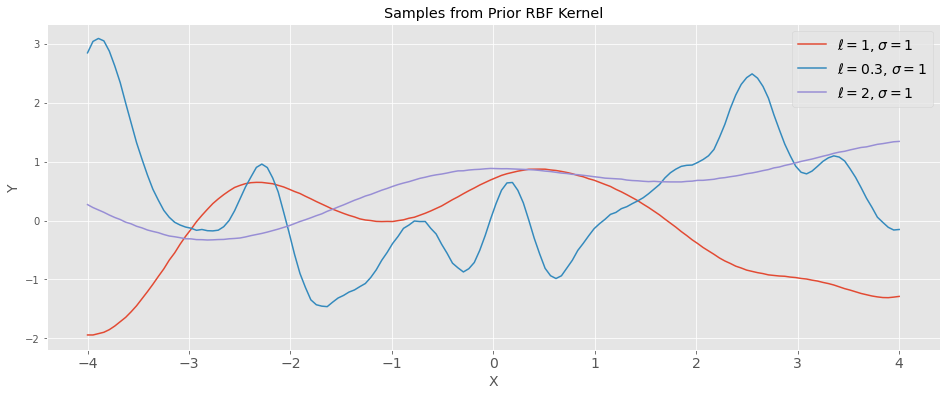
\includegraphics[scale=0.49]{images/samples_rbf_prior.png}
\caption{Three samples, each from an $RBF$ kernel with different hyperparameters denoted by the table legend. Notice how $\ell$ affects the smoothness of the function.}
\end{figure}

The \textit{periodic} ($Per$) kernel captures repeating structures, which can model seasonalities influenced by business cycles and or human behavior. For example, home electricity consumption often displays daily seasonalities. The \textit{periodic} kernel has the form

$$K_{per} = exp(-\frac{2}{\ell^2} sin^2 (\pi \frac{r}{p}))$$

where $p$ is the period. Again, $\ell$ and $\sigma^2$ are the lengthscale and outputscale respectively. Figure 2 below visualizes the repeating structures of the $Per$ kernel. Important in this thesis is how the period is chosen. In a time series, the correlation between any pair of outputs can be analyzed empirically using the Auto-correlation Function (ACF). The ACF compares the time series with itself at a certain lag. Namely:

\begin{figure}[htp]
\centering
\graphicspath{ {./images/} }
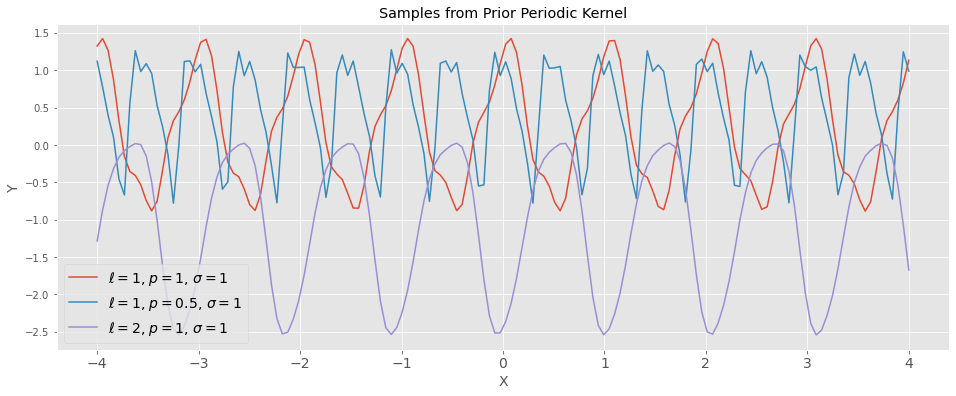
\includegraphics[scale=0.49]{images/samples_periodic_prior.png}
\caption{Three samples, each from a $Per$ kernel with different hyperparameters denoted by the table legend. Notice how $p$ affects the periodicity of the function and $\ell$ affects the "wiggliness" of the variations.}
\end{figure}

$$x + y + z$$

Thus, using the ACF, the interval of periods that show significant auto-correlation are chosen as the prior belief for the time series seasonality. Increasing the period $p$ increases the distance between repetitions. \textbf{Figure #.#} below shows an example of the ACF for the paper disposal machine.

The \textit{Rational Quadratic} ($RQ$) kernel can be interpreted as the sum of many $RBF$ kernels of different lengthscales. Similar to the $RBF$, the $RQ$ kernel encodes smoothness in the function space, but with the additional flexibility of having both local variations and long term variations. 

$$K_{RQ} = \sigma^2 exp(1 + \frac{(x - x')^2}{2\alpha \ell^2})$$

where $\alpha$, also known as the scale mixture, determines how much local variations from the smaller lengthscales contribute to the overall variation. By using this kernel, one can model non-periodic trends of the underlying physical process and interpret the hyperparameters $\ell$ as either a non-periodic hourly or daily trend depending on how large or small the value of $\ell$ is respectively. Three samples of the RQ kernel are visualized in Figure 3.

\begin{figure}[htp]
\centering
\graphicspath{ {./images/} }
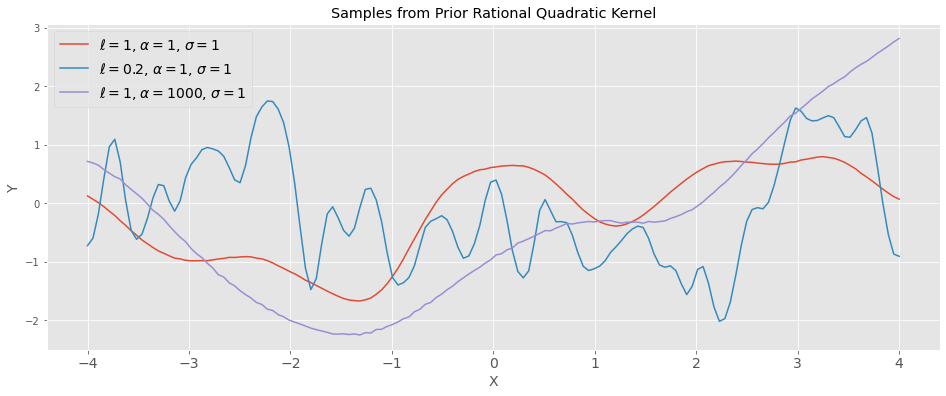
\includegraphics[scale=0.49]{images/samples_rq_prior.png}
\caption{Three samples, each from a $RQ$ kernel with different hyperparameters denoted by the table legend. Notice how $\alpha$ affects the . . . of the function and $\ell$ affects the "wiggliness" of the variations.}
\end{figure}




\textbf{Other}:

The main idea is as follows: we observe the function value at a fixed set of $N$ points, namely $y_n = f(x_n)$ for $n=1:N$, where $f$ is the unknown function. To predict the function value at a new point $x_*$, we have to compare how "similar" $x_*$ is to each of the $N$ training points. From there, we can predict that $f(x_*)$ is some weighted combinations of the $\{f(x_n)\}$ values.


\subsection{Advantages and Disadvantages of Gaussian Processes}

\subsection{Evaluation Metrics}